\documentclass[a4paper,12pt]{article}
\usepackage[utf8]{inputenc}
\usepackage[spanish]{babel}
\usepackage[T1]{fontenc}
\usepackage[dvips]{epsfig}
\usepackage[dvips]{graphicx}
\newcommand{\PI}{$\pi$}
\title{Número \PI}
\author{Zuleica Reina Segura}
\date{10/04/2014}
\begin{document}
\maketitle
\begin{abstract}
  \PI es la relación entre la longitud de una circunferencia y su diámetro, 
  en geometría euclidiana. Es un número irracional y una de las constantes matemáticas más importantes. 
  Se emplea frecuentemente en matemáticas, física e ingeniería.
\end{abstract}
\section{Primera sección}
El valor de \PI se ha obtenido con diversas aproximaciones a lo largo de la historia, 
siendo una de las constantes matemáticas que más aparece en las ecuaciones de la física, 
junto con el número e. Cabe destacar que el cociente entre la longitud de cualquier circunferencia 
y la de su diámetro no es constante en geometrías no euclídeas.
\section{Segunda sección}
Euclides fue el primero en demostrar que la relación entre una circunferencia y su diámetro 
es una cantidad constante.
\subsection{Historia}
La primera referencia que se conoce de \PI es aproximadamente del año 1650 adC en el Papiro de Ahmes, 
es un documento escrito en un papiro de unos seis metros de longitud y 33 cm de anchura, Contiene problemas 
matemáticos básicos, fracciones, cálculo de áreas, volúmenes, progresiones, repartos proporcionales, 
reglas de tres, ecuaciones lineales y trigonometría básica.
\cite{wikipedia}
\subsection{Definiciones analíticas}
\begin{itemize}
\item \PI es la relación entre la longitud de una circunferencia y su diámetro.
\item \PI es el área de un círculo unitario de radio unidad del plano euclídeo \footnote{Es un objeto ideal que solo posee dos dimensiones, y contiene infinitos puntos y rectas donde se satisfacen los axiomas de Euclides}.
\end{itemize}
\begin{figure}[htb]
\begin{center}
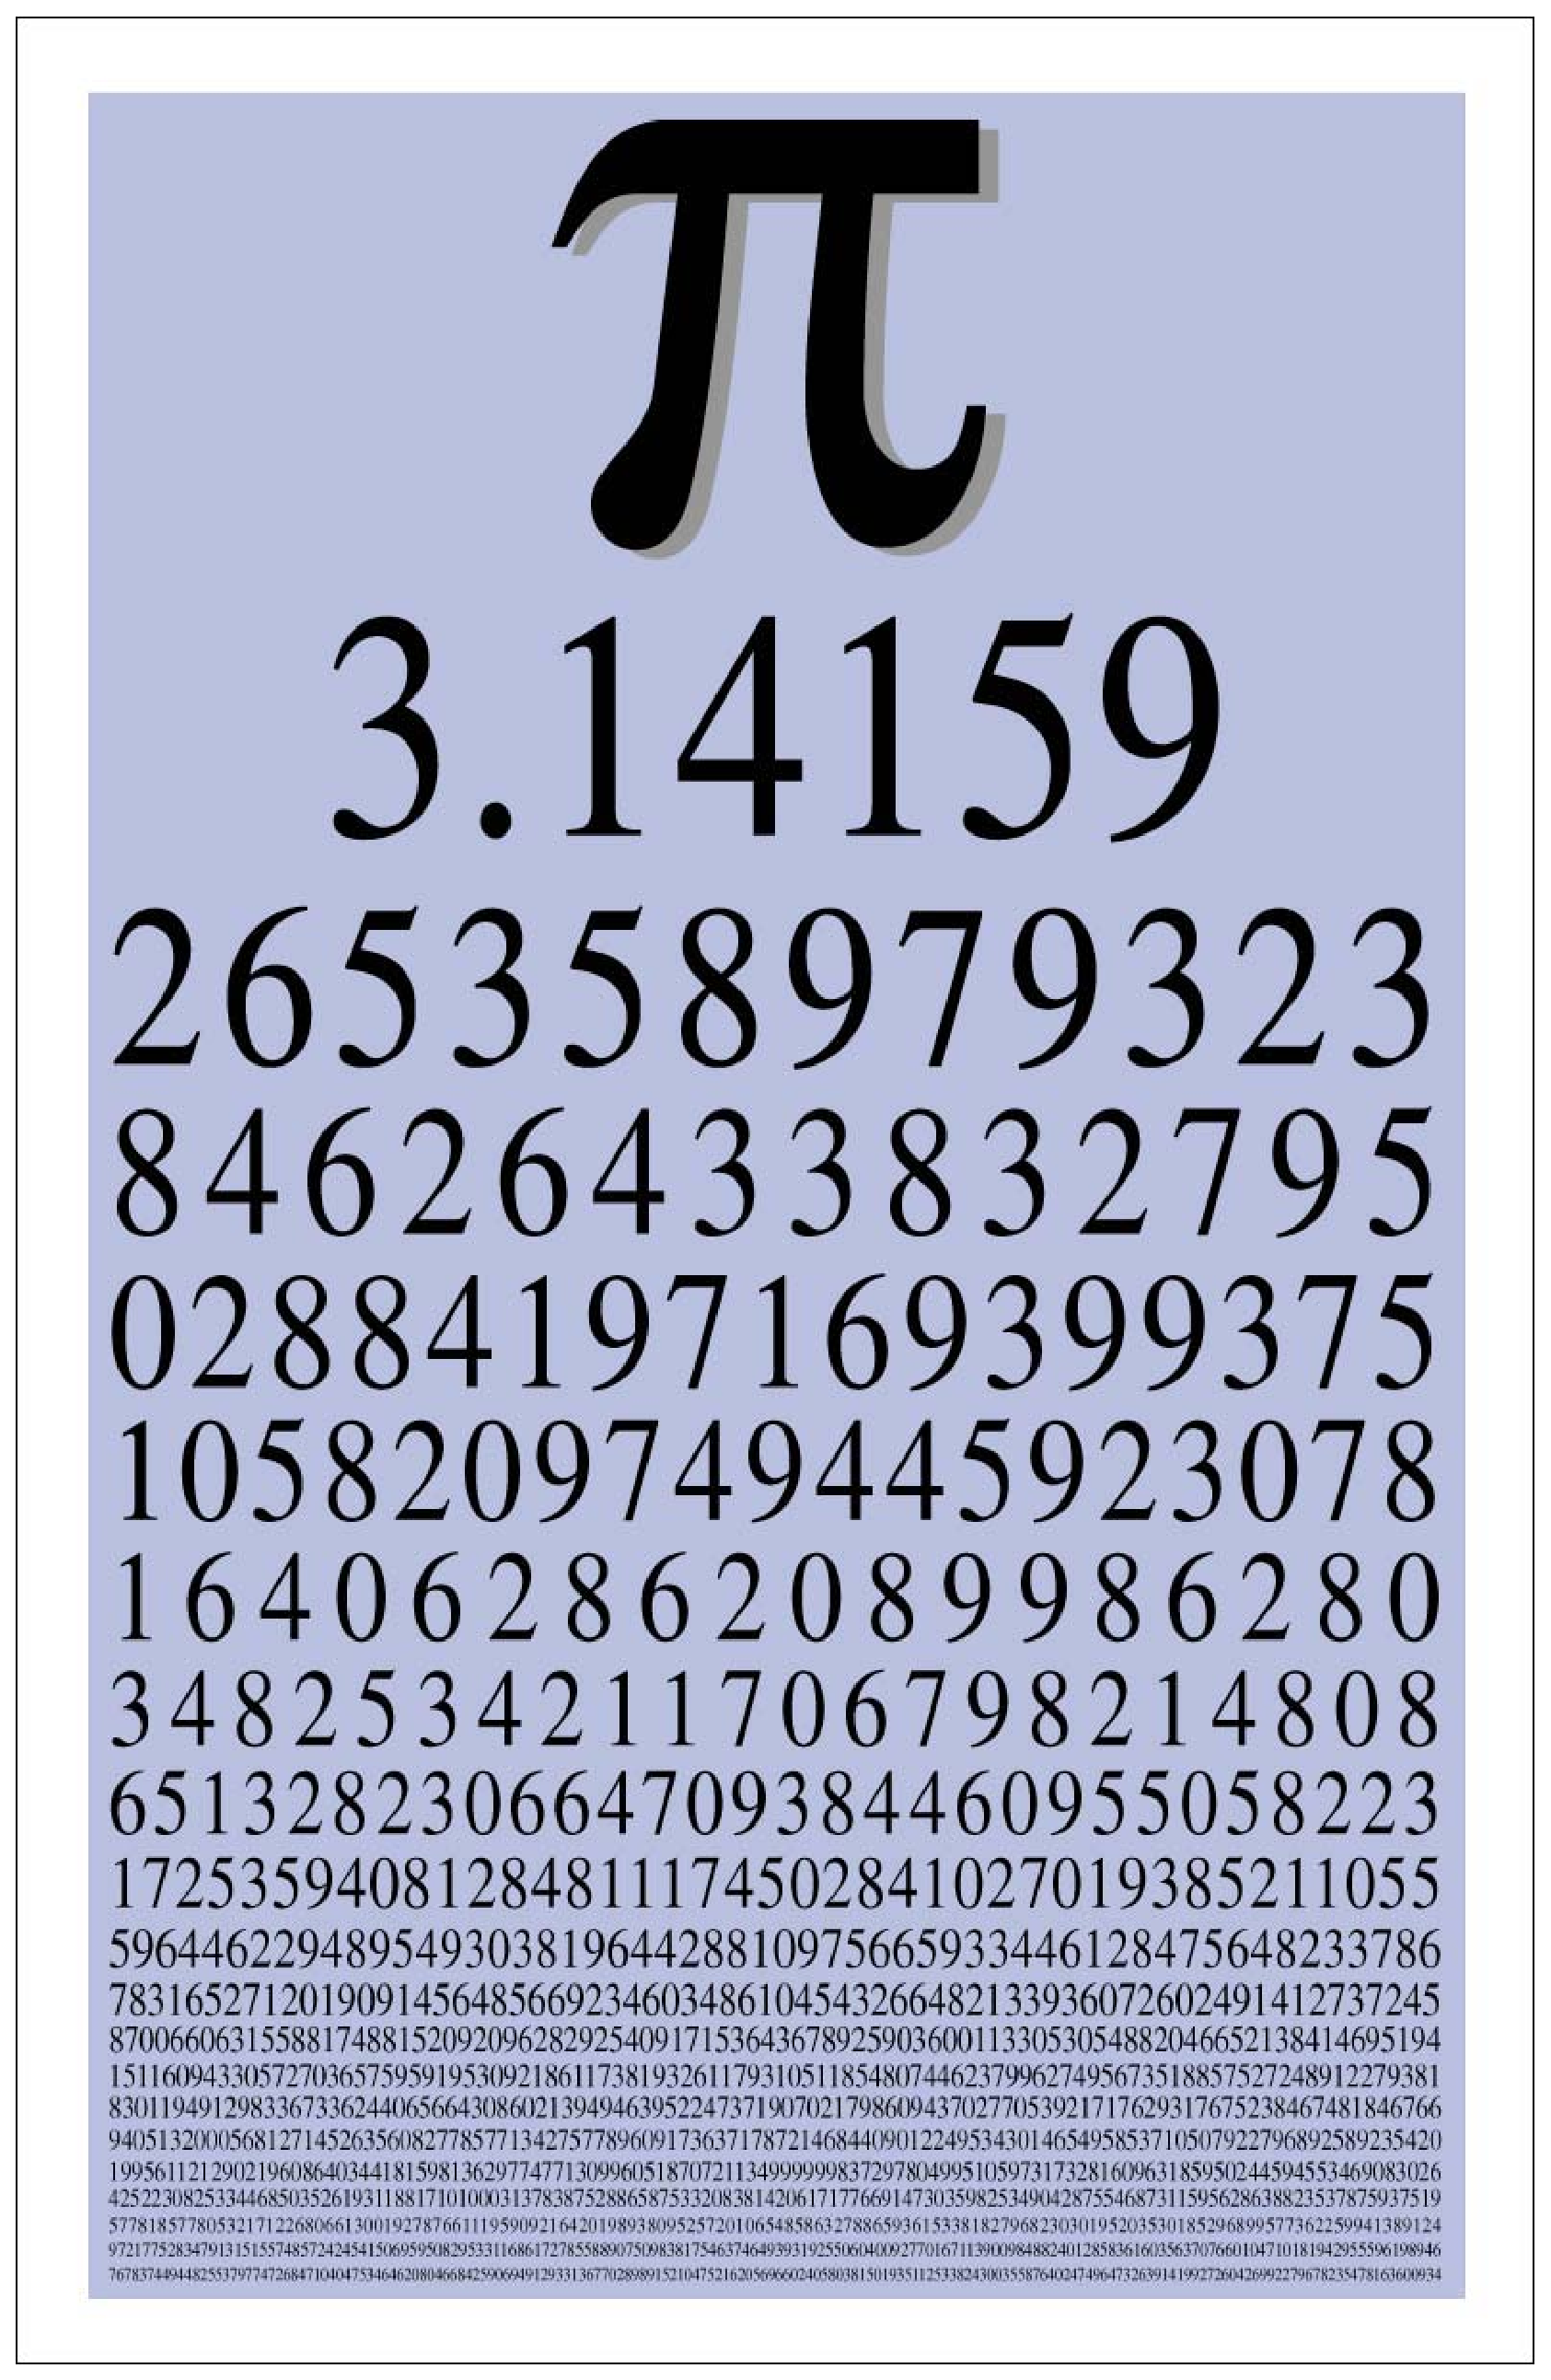
\includegraphics[width=0.5\textwidth]{images/figura1.eps}
\caption{Número \PI con varias cifras decimales}
\label{Número PI}
\end{center}
\end{figure}
\begin{table}[!ht]
\begin{tabular}{|l|c|c|}
\hline
Nombre & Año & Aproximación\\ \hline
Papiro de Ahmes & 1600 a.C. & 3.125 \\ \hline
Bandhayana & 500 a.C. & 3.09 \\ \hline
Liu Hui & 260 d.C. & 3.1416 \\ \hline
\end{tabular}
\caption{Aproximaciones del número \PI por diferentes autores durante la historia}
\label{tabla}
\cite{educacion}
\end{table}

\begin{thebibliography}{00}
\bibliography{bib/references}
\nocite{*}
\end{thebibliography}
\end{document}
